DIVERSES


\subsection{Bestimmung der geografischen Hierarchieebenen zu einer geografischen Position} 
			
			Jede der geografischen Hierarchieebenen beschreibt eine geografische Region.
			Liegt eine geografische Position beispielsweise innerhalb der geografischen Region eines Landes soll das zugehörige Land bestimmt werden können.

			Im Ortsverzeichnis von geonames.org sind die geografischen Regionen allerdings nicht hinterlegt.
			Jedes geografische Objekt wird hier durch eine geografische Position beschrieben.
			Es kann zu einer geografischen Position also nicht direkt bestimmt werden in welcher geografischen Region diese liegt.

			Es soll nun ein Vorgehen vorgestellt werden, welches es trotzdem ermöglicht für eine beliebige geografische Position alle geografischen Hierarchieebenen zu bestimmen.
			
			\subsubsection{Verfahren zur Bestimmung der geografischen Hierarchieebenen}

				In der geografischen Hierarchie wird der Globus am genauesten durch die geografischen Regionen der Städte eingeteilt.
				Durch die Teilmengenbeziehung der geografischen Hierarchie sind mit der Stadt implizit alle anderen Hierarchieebenen bestimmt.

				Deshalb soll eine geografische Position der am nächsten liegenden Stadt zugeordnet werden.
				Dadurch wird der Globus auf Städteebene in geografische Regionen eingeteilt. 
				Eine geografische Region zu einer Stadt S umfasst dann genau die Fläche, innerhalb der keine andere Stadt näher liegt als S.

				Diese Flächen werden auch Voronoi-Regionen genannt.

			\subsubsection{Voronoi-Diagramme} 

				Sei eine Menge von Punkten $Z = {z_1,z_2,...,z_n}$ auf einer Ebene verteilt.
				Eine Voronoi-Region $V^i$ zu einem Punkt $z_i$ beinhaltet dann alle Punkte $P^i={p_1,p_2,...,p_n}$ die näher an $z_i$ liegen als an allen anderen Punkten $Z_j={z_j in Z|z_j!=z_i}$.
				Alle Voronoi-Regionen zu allen Punkten in Z bilden ein Voronoi-Diagramm.

				Dieses Konzept kann zur Bestimmung der nächstgelegenen Stadt verwendet werden. 
				Die geografischen Positionen der Städte bilden dabei die Punkte $Z$.
				Zu jeder Stadt wird nun die Voronoi-Region erzeugt. 
				Anhand der Voronoi-Region in der ein Punkt p liegt kann nun bestimmt werden welche Stadt am nächsten zu p liegt.

				Jeder Punkt auf dem Globus kann so einer Stadt zugeordnet werden.
				Insbesondere wird der Globus auf Städteebene in geografische Regionen eingeteilt.
				In Abbildung \ref{img:voronoi} ist ein Voronoi-Diagramm einiger deutscher Städte dargestellt.

				\begin{figure}[h!]
				\begin{center}
				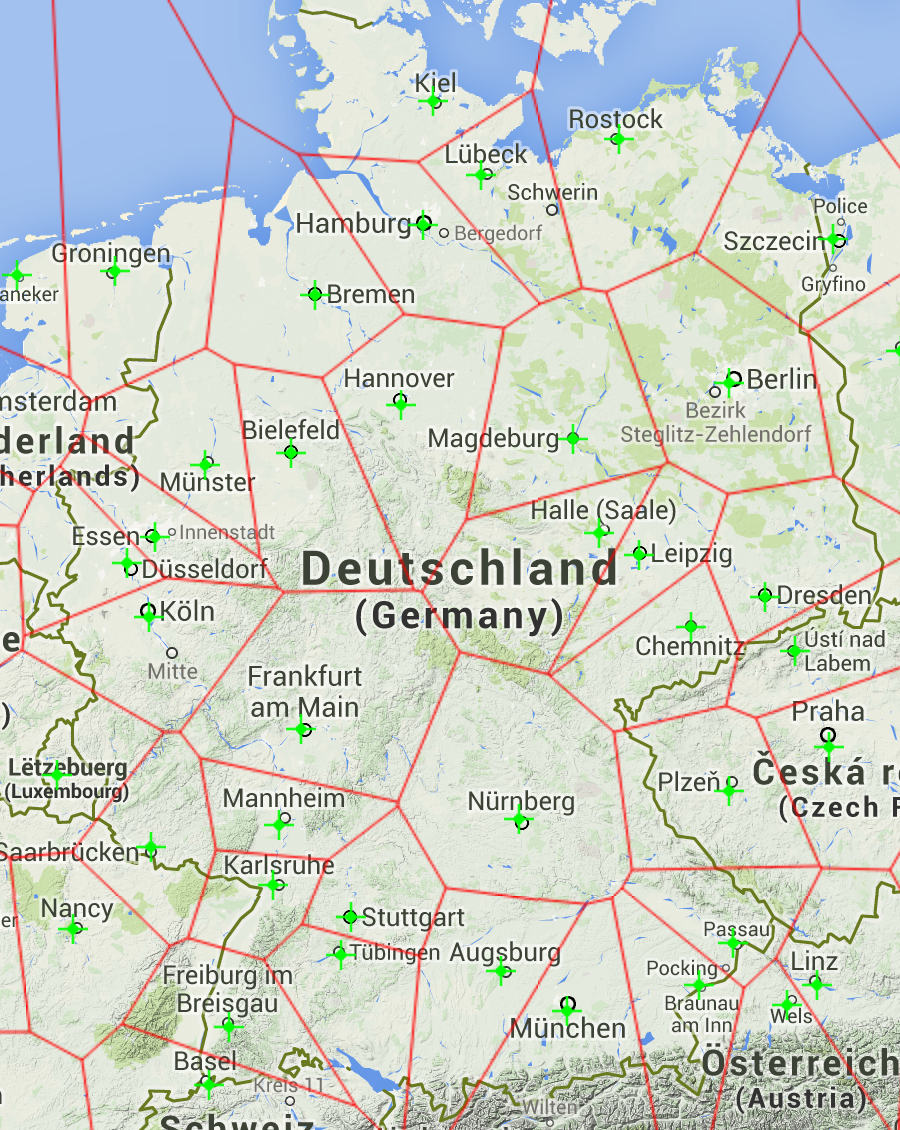
\includegraphics[scale=0.5]{voronoi.png}
				\caption{Vornoi-Diagramm Deutschland}
				\label{img:voronoi}
				\end{center}
				\end{figure}	

				Durch die Teilmengenbeziehung ist es nun nicht mehr nötig die geografischen Regionen der anderen Hierarchieebenen zu bestimmen.
				Es ist zu beachten, dass durch die Erzeugung der Vornoi-Regionen Ländergrenzen nur approximiert werden können. 
				Voronoi-Regionen zu Städten die in der Nähe einer Landesgrenze liegen können über die Landesgrenzen hinausgehen. 
				Damit werden geografische Positionen unter Umständen dem falschen Land zugeordnet.
				Auch dies ist in Abbildung \ref{img:voronoi} an den Landesgrenzen zu erkennen. 
				Umso größer allerdings die Anzahl der Städte ist, umso genauer wird die Approximation. 



\section{Tweet-Sammlung} 
		
		In der vorliegenden Arbeit werden zwei verschiedene Tweet-Sammlungen benutzt.
		Eine Tweet-Sammlung wird zum einlernen des Verfahrens genutzt.
		Diese Tweet-Sammlung die Daten sollen als Tweet-Lerndaten bezeichnet werden.
		Die andere Tweet-Sammlung beinhaltet eine Menge an Tweets um das Verfahren zu verifizieren.
		Diese werden Tweet-Kontrolldaten genannt.

		Im folgenden werden einige Kennzahlen zu den beiden Datensätzen aufgeführt.

		\paragraph{Tweet-Lerndaten} 

			Die Tweet-Lerndaten bestehen aus 383222 Datensätzen.
			Jeder Datensatz repräsentiert einen Tweet. 
			Die Datensätze beinhalten neben der Georeferenz in Form von Längen- und Breitengrad auch den Nutzer-Standort und die Nutzer-Zeitone des Verfassers.
			Die Tweets wurden im Zeitraum von 23.01.2014 bis 04.02.2014 über die Twitter Streaming Api gesammelt.

			Es wurden keine Tweets verwendet die vom selben Nutzer erstellt wurden. 
			Alle xyz Tweets in dieser Datenbasis stammen von unterschiedlichen Nutzern. 
			Damit soll eine Verzerrung der Ergebnisse vermieden werden.

		\paragraph{Tweet-Kontrolldaten}

			Diese Datenbasis beinhaltete 89692 Datensätze.
			Es sind dieselben Daten wie in der Tweet-Lerndaten Datenbasis vorhanden.
			Die Tweets wurden im Zeitraum vom 21.06.2013 bis 06.09.2013 über die Twitter Streaming Api gesammelt.

			Die Nutzer sind ebenfalls unterschiedlich und keiner der Nutzer kommt in der Tweet-Lerndaten Datenbasis vor.
